\documentclass[letterpaper,11pt,2p]{elsarticle}
%% The amssymb package provides various useful mathematical symbols
\usepackage{amssymb}
\usepackage{./Needed_Files/3dv}
\usepackage{times}
\usepackage{epsfig}
\usepackage{graphicx}
\usepackage{amsmath}
% Include other packages here, before hyperref.
% If you comment hyperref and then uncomment it, you should delete
% egpaper.aux before re-running latex.  (Or just hit 'q' on the first latex
% run, let it finish, and you should be clear).
\usepackage[pagebackref=true,breaklinks=true,letterpaper=true,colorlinks,bookmarks=false]{hyperref}
%\threedvfinalcopy % *** Uncomment this line for the final submission
\def\threedvPaperID{} % *** Enter the 3DV Paper ID here
\def\httilde{\mbox{\tt\raisebox{-.5ex}{\symbol{126}}}}

% Pages are numbered in submission mode, and unnumbered in camera-ready
\ifthreedvfinal\pagestyle{empty}\fi
\begin{document}
\begin{frontmatter}
\title{Team 1 - Final Paper}
%\tnotetext[label0]{This is only an example}
\author[]{Austin Vern Songer}
\author[]{Rozina Bahadur}
\author[]{Vincent Bruno}
\author[]{Nina Rodriguez}
\author[]{Olena Pushkar}
\author[]{Uma Rani}
\end{frontmatter}
\begin{center}
\textbf{ Robert Morris University - Capstone Project}
\end{center}
\begin{center}
\textbf{CLIENT: Body Fuel by Dana}
\end{center}


\newpage

\tableofcontents

\clearpage

\section{ EXECUTIVE SUMMARY}%%%%%%%%%%%%%%%%%%%%%%%%%%%%%%
\label{ES}%%%%%%%%%%%%%%%%%%%%%%%%%%%%%%%%%%%%%%%%%%%%%%%%

Body Fuel by Dana Renee was created in 2015 by Dana Bujalski, with the concept of helping busy individuals stick to their healthy eating goals. The business provides customers with pre-cooked and pre-measured plans based on amount of caloric intake or macros. Body Fuel by Dana Renee possessed an informational based website, which provided the customer with the menu, pricing, and order instructions. When we first meet with Ms.Bujalski orders were placed either through e-mail or telephone. She then took down the orders or stored them in her phone or e-mails.  Communication between her and her customers about new menus, order pickup, or invoices were sent through e-mail blasts, text messages or telephone calls. Payments were accepted through credit card services, PayPal, squarespace or she would accept cash.  Ms. Bujalski’s wanted an easier and efficient website that would integrate the customers into accounts on the new website which would store their meal plans and keep their orders store in a database, for easier management and delivery timelines. She also wanted a website that would allow to integrate her love for fitness and cooking, where she could host YouTube videos and teach others about a natural healthy lifestyle.\\


Ms.Bujalski is a colleague of one of the Vincent Bruno. We reached out to her because we knew she was a great fit for our capstone project for MIS590. When we introduce our concept and idea to Miss Dana she was astatic and eager to get started. The website was to be completed in 10 weeks and to presented and hand over the complete website to her at the end  of the 10 weeks.  Ms.Bujalski agreed to a \$300 dollar budget for the website and database implementation.\\

The completion of 10 weeks delivered a website, database, and analytics for Body Fuel by Dana Renee which integrated ecommerce subscription service, social media interactions, ability to updated and change the menus and pictures weekly, and customer service interactions with her customers in a timely manner for both her and her client in a more professional way.  Ms. Bujalski is on her way to generating revenue from Body Fuel and hopes to expand to a receipt e-book in the future.\\

\section{ INTRODUCTION}%%%%%%%%%%%%%%%%%%%%%%%%%%%%%%
\label{intro}%%%%%%%%%%%%%%%%%%%%%%%%%%%%%%%%%%%%%%%%%%%%%%%%

Organizations, enterprises, and associations today use the internet to provide information, conduct business transactions, and communicate with their customers. As technology keep becoming bigger and bigger, web based interaction have the potential to deliver small business opportunity to young entrepreneurs. Body Fuel by Dana Renee (BF), in Illinois, is interested in taking advantage of the simplicity and convenience of e commerce. She first needed our team to create custom integrated website that effectively communicated with an e commerce client. This would allow for her customers to pay for meal properly so that there is no miss payment upon arrival of the meals.   


\newpage 

\section{ BUSINESS ANALYSIS}%%%%%%%%%%%%%%%%%%%%%%%%%%%%%%
\label{BA}%%%%%%%%%%%%%%%%%%%%%%%%%%%%%%%%%%%%%%%%%%%%%%%%

Body Fuel by Dana Renee was created for busy individuals, who don’t have time to grocery shop, cook meals, and educate customers on a healthy eating lifestyle. Owner of Body Fuel, Dana Bujalski started her business in 2015 and has been operating on her own for eight months. Dana is a trained Chef with her Culinary Art degree with several years of industry and professional chef experience. She is her own living testament as she is her own example of clean eating and fitness. She competes in bikini competitions around the country with her goal to obtain her pro card in the near future.  Body Fuel’s motto is “There is no diet that will do what eating healthy does” (2016 Body Fuel).\\ 

Body Fuel by Dana Renee provides customers with homemade then packaged healthy foods so that busy individual can stick to their fitness goals without all the fuss of worry when they will have time to meal prep. Her meals are made with fresh, local organic ingredients. They are free of gluten, refined sugars, antibiotics, hormones and GMO.  Customers can either choose the 21 meal plan which includes seven breakfast and 14 entrees or customize their own plan with a minimum of 10 meals. The menu changes weekly depending on which items are in season.  The tone-up plan costs \$203.00 and the Fuel-up is \$240.00. \\

Meals are cooked on Wednesday in a rented sanitized industrial local kitchen. The meals are then packed in easily stackable containers that are FDA approved, 100\% recyclable, microwavable, freezer and dishwasher safe.  Deadline for order placement is by 7PM on Mondays.  Food can be picked up in St. Charles on Friday of the same week from 8AM until 6PM. Payments accepted are Credit Card, PayPal, or cash. Shelf life is 6 days from the day of delivery.\\


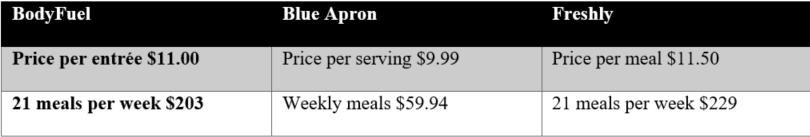
\includegraphics[scale=0.9]{Compare}\\


Body Fuel by Dana Renee meal plans are lower in cost in comparison to her competitors.  Freshly offers \$11.50 per meal and \$229 for 21meals (2015, Freshly, meals). Blue Apron offers a 2 serving meal for \$9.99 and a weekly cost of \$59.95 (2015, Blue Apron). Body Fuel meal plans range from \$203.00 to \$240.00 for 21 meals and \$9-\$11 dollars per meal (2016, Body fuel, meals).

\begin{center}
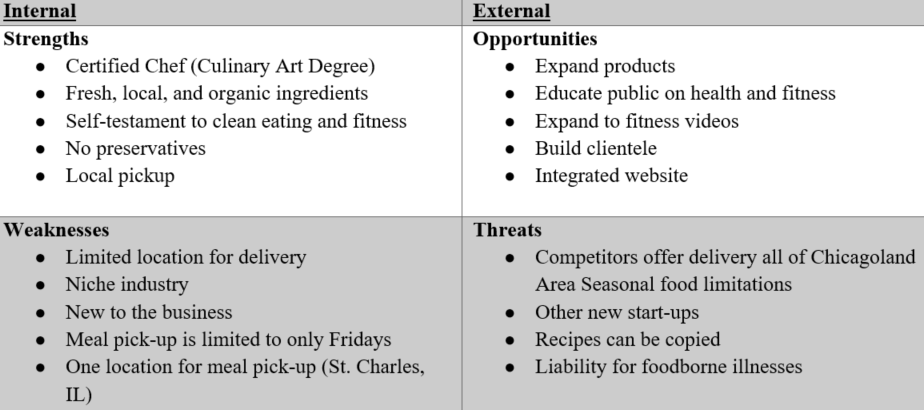
\includegraphics[scale=0.6]{SWOT}\\
\end{center}



%=============================================
\subsection{ Scope of Work}%=======================
\label{subsec1}%==============================

Dana Bujalski met with our team to discuss the business goals of Body Fuel and what she would like to accomplish in joining with our team. Her goal is to have an interactive website that will streamline the ease of ordering process, retain client information, accept online payments that are disbursed directly to her account, and integrate social media accounts to keep her customers up to date in the life of Dana Bujalski. Ms. Bujalski currently handles all her orders by telephone or e-mails, where she writes down the information on paper or through her notes application on her phone.  She sends e-mail blasts and text message up dates to her clients about order reminders, deadlines, and meal delivery.\\

The site did not meet Dana’s aspiration to build relationships with customers and it did not reflect innovative advances in today's technology. The principle goal of this project is to upgrade Body Fuel’s website and database management system that not just updates to today's technologies and web base clients, but also likewise communicate effectively with its customers. Additional goals to support her main goal include the following:

\begin{itemize}
    \item To store her customer’s e-mails and meal plan information which will allow her to send them weekly updates.
    \item Create automated alerts and blasts
    \item Integration for YouTube videos and other social media
    \begin{itemize}
        \item Videos of her cooking, fitness, and other fitness subjects.
        \item Ability to easily update her website to change the menus and also to list nutritional facts of foods prepped ingredients, macros, calories, etc.
    \end{itemize}
\end{itemize}

These specific goals require the utilization of rich media content, specifically the utilization of video and sound substance, through which customers would be able to listen or watch the recordings. The site needed to give the important urgent data and additionally keep up with the new up and coming content for continued success for the future. 




%=============================================
\subsection{ Current State Analysis}
\label{subsec1}





%=============================================
\subsection{ Requirements}
\label{subsec1}





%=============================================
\subsection{ Solution \& Scope}
\label{subsec1}





%=============================================
\subsubsection{ Deliverables}
\label{subsec1}





%=============================================
\subsection{ Cost}
\label{subsec1}





%=============================================
\subsection{ Constraints}
\label{subsec1}




\section{ DEVELOPMENT}%%%%%%%%%%%%%%%%%%%%%%%%%%%%%%%%%%%%
\label{FEA}%%%%%%%%%%%%%%%%%%%%%%%%%%%%%%%%%%%%%%%%%%%%%%%



%=============================================
\subsection{ Team}
\label{subsec1}


%=============================================
\subsubsection{ IS Consulting Team Lead}
\label{subsec1}

%=============================================
\subsubsection{ Client Liaison \& Representative }
\label{subsec1}

%=============================================
\subsubsection{ Business Analysis}
\label{subsec1}

%=============================================
\subsubsection{ Technical Design}
\label{subsec1}

%=============================================
\subsubsection{ Implementation Plan}
\label{subsec1}


%=============================================
\subsection{ Development Tools}
\label{subsec1}


%=============================================
\subsubsection{ Github}
\label{subsec1}


%=============================================
\subsubsection{ Slack}
\label{subsec1}







\newpage 

\section{ TECHNICAL DESIGN}%%%%%%%%%%%%%%%%%%%%%%%%%%%%%%%
\label{TD}%%%%%%%%%%%%%%%%%%%%%%%%%%%%%%%%%%%%%%%%%%%%%%%%

The original Body Fuel by Dana Renee website was hosted by Squarespace where they host both personal and business websites. Squarespace gave Dana minimal ability to update and personalize the website to her needs which added her to reach out and search for a new option.  One of Dana’s goals was that she wanted the ability to update her own website to change the menus weekly, update ingredients, and add videos content and downloads.  Our team brainstormed and researched a few websites and decided the best option was for Dana to use WordPress. WordPress is ideal for any size businesses according to an article by Shubhomita Bose for Small Business Trends, many users have said that WordPress is reliable and has built trust, user friendly, and has built trust among business owners (2016, para. 2). Our team was also able to procure several free templates to design the site. The color scheme was chosen by Ms.Bujalski and the team members who voted on several options. \\

\begin{center}
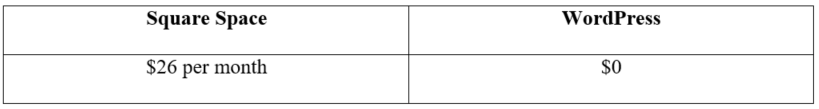
\includegraphics[scale=0.7]{Platform}\\
\end{center}

WordPress is the cheaper option for the project and maximizes customer value for small businesses. WordPress will also allow Ms.Bujalski capability to update and add content to the site since it is more a small business friendly. Only fee that will be associated is the host fee to run the site which there are plans from \$5 dollars a month and up.\\

%=============================================
\subsection{Web Platform - Wordpress}
\label{subsec1}


\subsubsection{Plugins}
%=========
\medskip
{\large WooCommerce }



\medskip
{\large WooCommerce API Manager}



\medskip
{\large WooCommerce Social Login}



\medskip
{\large WooCommerce Slack}



\medskip
{\large All in One WP Security}



\medskip
{\large W3 Total Cache}



\medskip
{\large Google XML Sitemaps}




\medskip
{\large Facebook Auto Post}





%=============================================
\subsection{ Web Application Framework}
\label{subsec1}





%=============================================
\subsection{ Web Server}
\label{subsec1}





%=============================================
\subsection{ Infrastructure}
\label{subsec1}





%=============================================
\subsubsection{ Hosting}
\label{subsec1}





%=============================================
\subsubsection{ 3rd Party API Integration}
\label{subsec1}





%=============================================
\subsubsection{ Data Encryption}
\label{subsec1}





%=============================================
\subsection{ Analytics and Tracking}
\label{subsec1}





%=============================================
\subsection{ Email Services}
\label{subsec1}





%=============================================
\subsection{ SSL}
\label{subsec1}





%=============================================
\subsection{ Javascript Libraries}
\label{subsec1}





%=============================================
\subsection{ Database}
\label{subsec1}





%=============================================
\subsubsection{ ER Diagram}
\label{subsec1}





%=============================================
\subsection{ Database Manager}
\label{subsec1}





%=============================================
\subsection{ Security}
\label{subsec1}




\newpage 


%%%%%%%%%%%%%%%%%%%%%%%%%%%%%%%%%%%%%%%%%%%%%%%%%%%%%%%%%%
%%%%%%%%%%%%%%%%%%%%%%%%%%%%%%%%%%%%%%%%%%%%%%%%%%%%%%%%%%
\section{IMPLEMENTATION PLAN}



%=============================================
\subsection{ Phase 01 - Testing \& Delivery}
\label{subsec1}




%=============================================
\subsection{ Phase 02 - Maintenance}
\label{subsec1}



\newpage 

%%%%%%%%%%%%%%%%%%%%%%%%%%%%%%%%%%%%%%%%%%%%%%%%%%%%%%%%%%
%%%%%%%%%%%%%%%%%%%%%%%%%%%%%%%%%%%%%%%%%%%%%%%%%%%%%%%%%%
\section{CONCLUSION}
\label{subsec1}


\newpage 

%%%%%%%%%%%%%%%%%%%%%%%%%%%%%%%%%%%%%%%%%%%%%%%%%%%%%%%%%%
%%%%%%%%%%%%%%%%%%%%%%%%%%%%%%%%%%%%%%%%%%%%%%%%%%%%%%%%%%
\section{REFERENCES}
\label{subsec1}


\newpage 


%%%%%%%%%%%%%%%%%%%%%%%%%%%%%%%%%%%%%%%%%%%%%%%%%%%%%%%%%%
%%%%%%%%%%%%%%%%%%%%%%%%%%%%%%%%%%%%%%%%%%%%%%%%%%%%%%%%%%
\section{APPENDIX a}
\label{subsec1}







%% The Appendices part is started with the command \appendix;
%% appendix sections are then done as normal sections
%\appendix

%\section{Section in Appendix}
%\label{appendix-sec1}

%Sample text. Sample text. Sample text. Sample text. Sample text. Sample text. 
%Sample text. Sample text. Sample text. Sample text. Sample text. Sample text. 
%Sample text. 

%% References
%%
%% Following citation commands can be used in the body text:
%% Usage of \cite is as follows:
%%   \cite{key}         ==>>  [#]
%%   \cite[chap. 2]{key} ==>> [#, chap. 2]
%%

%% References with bibTeX database:

% \bibliographystyle{elsarticle-num}
% \bibliographystyle{elsarticle-harv}
% \bibliographystyle{elsarticle-num-names}
% \bibliographystyle{model1a-num-names}
% \bibliographystyle{model1b-num-names}
% \bibliographystyle{model1c-num-names}
% \bibliographystyle{model1-num-names}
% \bibliographystyle{model2-names}
% \bibliographystyle{model3a-num-names}
% \bibliographystyle{model3-num-names}
% \bibliographystyle{model4-names}
% \bibliographystyle{model5-names}
% \bibliographystyle{model6-num-names}

%\bibliography{sample}


\end{document}

%%
%% End of file `elsarticle-template-num.tex'.
